\documentclass[11pt,compress,t,notes=noshow]{beamer}
\usepackage[]{graphicx}\usepackage[]{color}
% maxwidth is the original width if it is less than linewidth
% otherwise use linewidth (to make sure the graphics do not exceed the margin)
\makeatletter
\def\maxwidth{ %
  \ifdim\Gin@nat@width>\linewidth
    \linewidth
  \else
    \Gin@nat@width
  \fi
}
\makeatother

\definecolor{fgcolor}{rgb}{0.345, 0.345, 0.345}
\newcommand{\hlnum}[1]{\textcolor[rgb]{0.686,0.059,0.569}{#1}}%
\newcommand{\hlstr}[1]{\textcolor[rgb]{0.192,0.494,0.8}{#1}}%
\newcommand{\hlcom}[1]{\textcolor[rgb]{0.678,0.584,0.686}{\textit{#1}}}%
\newcommand{\hlopt}[1]{\textcolor[rgb]{0,0,0}{#1}}%
\newcommand{\hlstd}[1]{\textcolor[rgb]{0.345,0.345,0.345}{#1}}%
\newcommand{\hlkwa}[1]{\textcolor[rgb]{0.161,0.373,0.58}{\textbf{#1}}}%
\newcommand{\hlkwb}[1]{\textcolor[rgb]{0.69,0.353,0.396}{#1}}%
\newcommand{\hlkwc}[1]{\textcolor[rgb]{0.333,0.667,0.333}{#1}}%
\newcommand{\hlkwd}[1]{\textcolor[rgb]{0.737,0.353,0.396}{\textbf{#1}}}%
\let\hlipl\hlkwb

\usepackage{framed}
\makeatletter
\newenvironment{kframe}{%
 \def\at@end@of@kframe{}%
 \ifinner\ifhmode%
  \def\at@end@of@kframe{\end{minipage}}%
  \begin{minipage}{\columnwidth}%
 \fi\fi%
 \def\FrameCommand##1{\hskip\@totalleftmargin \hskip-\fboxsep
 \colorbox{shadecolor}{##1}\hskip-\fboxsep
     % There is no \\@totalrightmargin, so:
     \hskip-\linewidth \hskip-\@totalleftmargin \hskip\columnwidth}%
 \MakeFramed {\advance\hsize-\width
   \@totalleftmargin\z@ \linewidth\hsize
   \@setminipage}}%
 {\par\unskip\endMakeFramed%
 \at@end@of@kframe}
\makeatother

\definecolor{shadecolor}{rgb}{.97, .97, .97}
\definecolor{messagecolor}{rgb}{0, 0, 0}
\definecolor{warningcolor}{rgb}{1, 0, 1}
\definecolor{errorcolor}{rgb}{1, 0, 0}
\newenvironment{knitrout}{}{} % an empty environment to be redefined in TeX

\usepackage{alltt}
\newcommand{\SweaveOpts}[1]{}  % do not interfere with LaTeX
\newcommand{\SweaveInput}[1]{} % because they are not real TeX commands
\newcommand{\Sexpr}[1]{}       % will only be parsed by R



\usepackage[english]{babel}
\usepackage{dsfont}
\newcommand\bmmax{2}
\usepackage{bm}
\usepackage{bbm}
\usepackage{verbatim}
\usepackage{amsmath}
\usepackage{amsfonts}
\usepackage{csquotes}
\usepackage{multirow}
\usepackage{longtable}
\usepackage{enumerate}
\usepackage[absolute,overlay]{textpos}
\usepackage{psfrag}
\usepackage{algorithm}
\usepackage{algorithmicx}
\usepackage{algpseudocode}
\usepackage{eqnarray}
\usepackage{multimedia}
\usepackage{media9}
\usepackage{arydshln}
\usepackage{tabularx}
\usepackage{placeins}
\usepackage{tikz}
\usepackage{setspace}
\usepackage{wrapfig}
\usepackage{tcolorbox}
\usepackage[export]{adjustbox}
\usepackage{siunitx}
\usetikzlibrary{shapes,arrows,automata,positioning,calc}
\def\signed #1{{\leavevmode\unskip\nobreak\hfil\penalty50\hskip1em
  \hbox{}\nobreak\hfill #1%
  \parfillskip=0pt \finalhyphendemerits=0 \endgraf}}

\newsavebox\mybox
\newenvironment{aquote}[1]
  {\savebox\mybox{#1}\begin{quote}\openautoquote\hspace*{-.7ex}}
  {\unskip\closeautoquote\vspace*{1mm}\signed{\usebox\mybox}\end{quote}}
  
\tikzset{
  %Define standard arrow tip
  >=stealth',
  %Define style for boxes
  punkt/.style={
    rectangle,
    rounded corners,
    draw=black, very thick,
    text width=6.5em,
    minimum height=2em,
    text centered},
  % Define arrow style
  pil/.style={
    ->,
    thick,
    shorten <=2pt,
    shorten >=2pt,}
}
\usepackage{subfig}

%new environments

\newenvironment{vbframe}  %frame with breaks and verbatim
{
 \begin{frame}[containsverbatim,allowframebreaks]
}
{
\end{frame}
}

\newenvironment{vframe}  %frame with verbatim without breaks (to avoid numbering one slided frames)
{
 \begin{frame}[containsverbatim]
}
{
\end{frame}
}

\newenvironment{blocki}[1]   % itemize block
{
 \begin{block}{#1}\begin{itemize}
}
{
\end{itemize}\end{block}
}

\newenvironment{fragileframe}[2]{  %fragile frame with framebreaks
\begin{frame}[allowframebreaks, fragile, environment = fragileframe]
\frametitle{#1}
#2}
{\end{frame}}


\newcommand{\myframe}[2]{  %short for frame with framebreaks
\begin{frame}[allowframebreaks]
\frametitle{#1}
#2
\end{frame}}

\newcommand{\remark}[1]{
  \textbf{Remark:} #1
}

%%%%%%%%%%%%%%%%%%%%%%%%%%%%%%%%%%%%%%%%%%%%%%%%%%%%%%%%%%%%%%%%%%%%%%%%%%%%%%%

% basic latex stuff
\newcommand{\pkg}[1]{{\fontseries{b}\selectfont #1}} %fontstyle for R packages
\newcommand{\lz}{\vspace{0.5cm}} %vertical space
\newcommand{\dlz}{\vspace{1cm}} %double vertical space
\newcommand{\oneliner}[1] % Oneliner for important statements
{\begin{block}{}\begin{center}\begin{Large}#1\end{Large}\end{center}\end{block}}


%\usetheme{lmu-lecture}
\usepackage{../style/lmu-lecture}

\let\code=\texttt
\let\proglang=\textsf

\setkeys{Gin}{width=0.9\textwidth}



\title{Introduction to Machine Learning}
\author{Bernd Bischl}
\institute{Department of Statistics -- LMU Munich}
\date{Winter term 2021}

\setbeamertemplate{frametitle}{\expandafter\uppercase\expandafter\insertframetitle}



\begin{document}
%This file is a child of preamble.Rnw in the style folder
%if you want to add stuff to the preamble go there to make
%your changes available to all childs





\input{../latex-math/basic-math}
\input{../latex-math/basic-ml}
\input{../latex-math/ml-nn}


\lecturechapter{3}{Deep Learning- MLP}
\lecture{Deep Learning- MLP}
%%%%%%%%%%%%%%%%%%%%%%%%%%%%%%%%%%%%%%%%%%%%%%%%%%%%%%%%%%%%%%%%%%

\begin{vbframe}{Motivation}
\begin{itemize}
\item We have a nice graphical way of representing simple functions/models like logistic regression. Why is that useful?
\item It is useful because this visual metaphor allows us to use such individual neurons as building blocks of considerably more complicated functions.
\item Therefore, networks of neurons can represent extremely complex hypothesis spaces.
\item Most importantly, it allows us to define the \enquote{right} kinds of hypothesis spaces to learn functions that are more common in our universe in a data-efficient way (see Lin, Tegmark et al. 2016).
\end{itemize}
\end{vbframe}
%%%%%%%%%%%%%%%%%%%%%%%%%%%%%%%%%%%%%%%%%%%%%%%%%%%%%%%%%%%%%%%%%%

\begin{frame} {Motivation}
\begin{itemize}
\item \small{But why do we need more complicated functions? Is logistic regression not enough?}
\item \small{Because a single neuron is restricted to learning only linear decision boundaries, its performance on the task below will be quite poor. }
\begin{figure}
\centering
\scalebox{0.25}{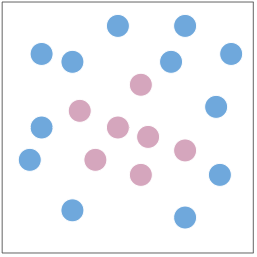
\includegraphics{plots/cartesian.png}}
\end{figure}
\item \small{However, if the original features are transformed (for example from Cartesian to polar coord.), the neuron can easily separate the classes.}
\begin{figure}
\centering
\scalebox{0.25}{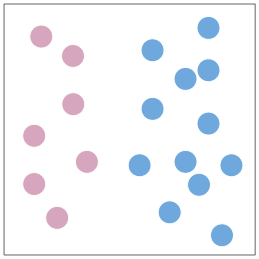
\includegraphics{plots/polar.png}}
\end{figure}
\end{itemize}
\end{frame}
%%%%%%%%%%%%%%%%%%%%%%%%%%%%%%%%%%%%%%%%%%%%%%%%%%%%%%%%%%%%%%%%%%

\begin{frame} {Motivation}
  \small{Instead of classifying the data in the original representation, ...}
    \begin{figure}
    \centering
      \scalebox{1}{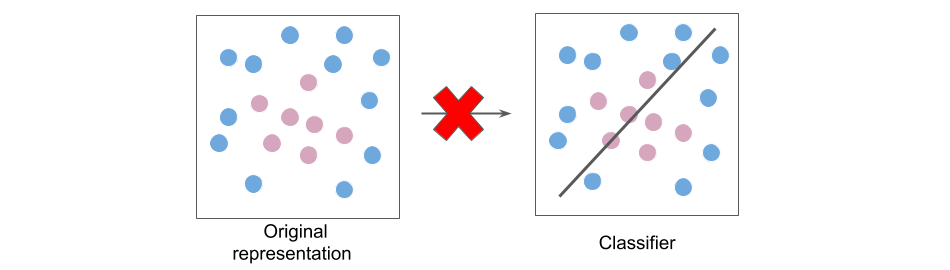
\includegraphics{plots/repold_f.png}}
  \end{figure}
\end{frame}
%%%%%%%%%%%%%%%%%%%%%%%%%%%%%%%%%%%%%%%%%%%%%%%%%%%%%%%%%%%%%%%%%%

\begin{frame} {Motivation}
   \small{we classify it in the new feature space.}
  \begin{figure}
    \centering
      \scalebox{1}{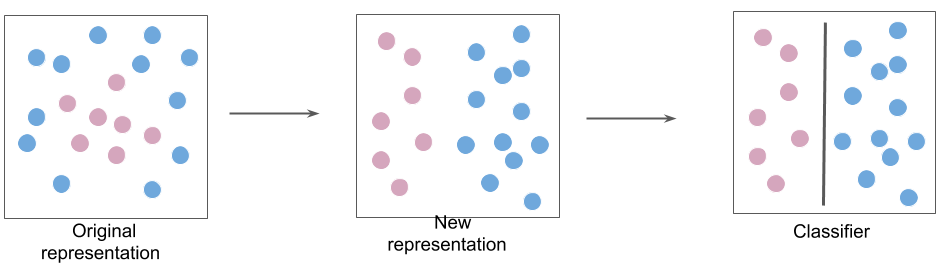
\includegraphics{plots/repnew_f.png}}
  \end{figure}
\end{frame}
%%%%%%%%%%%%%%%%%%%%%%%%%%%%%%%%%%%%%%%%%%%%%%%%%%%%%%%%%%%%%%%%%%

\begin{frame} {Motivation}
   \small{we classify it in the new feature space.}
  \begin{figure}
    \centering
      \scalebox{1}{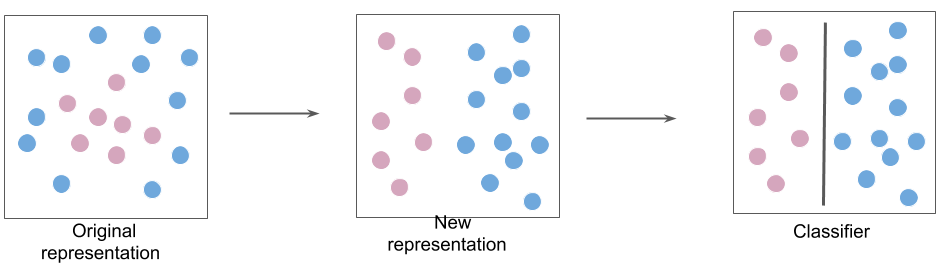
\includegraphics{plots/repnew_f.png}}
  \end{figure}
  \small{Analogously, }
  \begin{figure}
    \centering
      \scalebox{0.75}{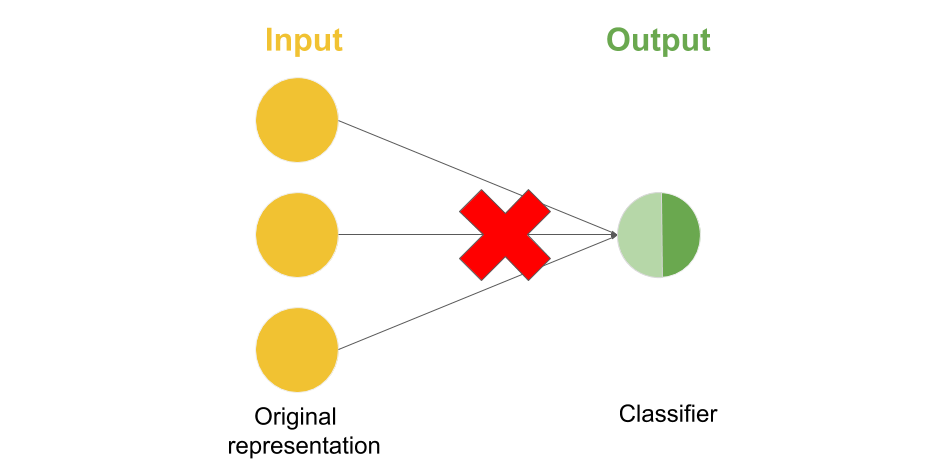
\includegraphics{plots/oldrep_n_f.png}}
  \end{figure}
\end{frame}
%%%%%%%%%%%%%%%%%%%%%%%%%%%%%%%%%%%%%%%%%%%%%%%%%%%%%%%%%%%%%%%%%%

\begin{frame} {Motivation}
   \small{we classify it in the new feature space.}
  \begin{figure}
    \centering
      \scalebox{1}{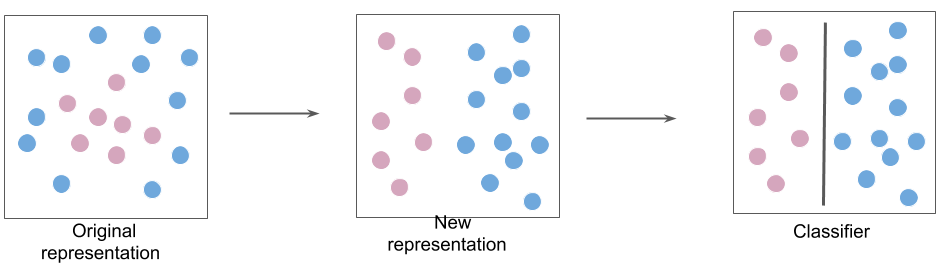
\includegraphics{plots/repnew_f.png}}
  \end{figure}
  \small{Analogously, }
  \begin{figure}
    \centering
      \scalebox{0.75}{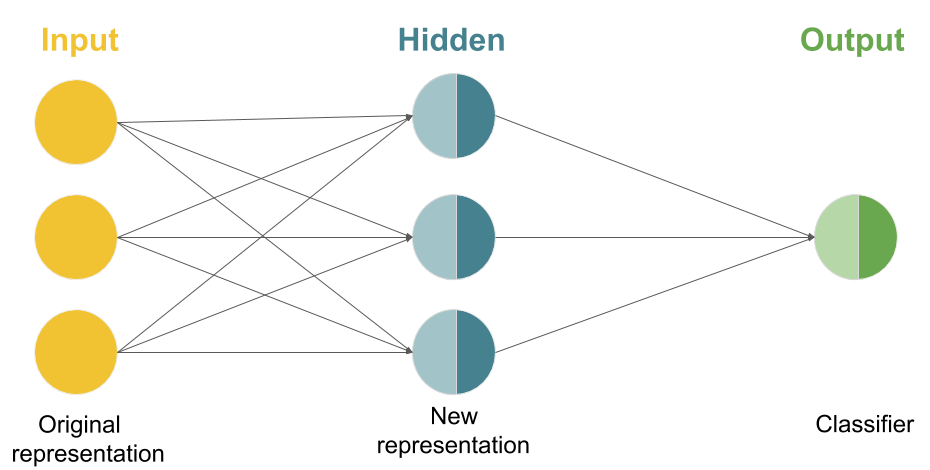
\includegraphics{plots/newrep_n_f.png}}
  \end{figure}
\end{frame}
%%%%%%%%%%%%%%%%%%%%%%%%%%%%%%%%%%%%%%%%%%%%%%%%%%%%%%%%%%%%%%%%%%

\begin{frame} {Representation Learning}
  \begin{itemize}
    \vspace{5mm}
    \item Therefore, it is \textit{very} critical to feed a classifier the \enquote{right} features in order for it to perform well.
    \vspace{7mm}
    \item Before deep learning (DL) took off, features for tasks like machine vision and speech recognition were \enquote{hand-designed} by domain experts. This step of the machine learning pipeline is called \textbf{feature engineering}.
    \vspace{7mm}
    \item The single biggest reason DL is so important is that it automates feature engineering. This is called \textbf{representation learning}.
  \end{itemize}
\end{frame}
%%%%%%%%%%%%%%%%%%%%%%%%%%%%%%%%%%%%%%%%%%%%%%%%%%%%%%%%%%%%%%%%%%

\begin{vbframe} {Single Hidden Layer Networks}
\begin{itemize}
\item The input $\xv$ is a column vector with dimensions $p \times 1$. 
\item $\Wmat$ is a weight matrix with dimensions $p \times m$:
$$\Wmat =\begin{pmatrix}
      w_{1,1} & w_{1,2} & \cdots & w_{1,m} \\
      w_{2,1} & w_{2,2} & \cdots & w_{2,m} \\
      \vdots  & \vdots  & \ddots & \vdots  \\
      w_{p,1} & w_{p,2} & \cdots & w_{p,m}\end{pmatrix}$$
\item For example, to obtain $z_1$, we pick the first column of $W$:
$$\Wmat_1 =\begin{pmatrix}
      w_{1,1} \\
      w_{2,1} \\
      \vdots  \\
      w_{p,1}\end{pmatrix}$$
    and compute $z_1 = \sigma(W_1^\top \xv + b_1)$, where $b_1$ is the bias of the first hidden neuron and $\sigma: \R \to \R$ is an activation function. 
\end{itemize}
\end{vbframe}
%%%%%%%%%%%%%%%%%%%%%%%%%%%%%%%%%%%%%%%%%%%%%%%%%%%%%%%%%%%%%%%%%%

\begin{vbframe}{Single Hidden Layer Networks: Notation}
  \textbf{General notation}:
  \begin{itemize}
    \vspace{4mm}
    \item The network has $m$ hidden neurons $z_1, \dots, z_m$ with
    $$ z_j = \sigma(\Wmat_j^\top \xv + b_j)$$
    \vspace{-0.5cm}
    \begin{itemize}
    \item $z_{in,j}  = \Wmat_j^\top \xv + b_j$
    \vspace{2mm}
    \item $z_{out,j} = \sigma(z_{in,j}) = \sigma(\Wmat_j^\top \xv + b_j)$
    \end{itemize}
    \vspace{4mm}
    for $j \in \{1,\ldots,m\}$.
    \vspace{4mm}
\framebreak 
%%%%%%%%%%%%%%%%%%%%%%%%%%%%%%%%%%%%%%%%%%%%%%%%%%%%%%%%%%%%%%%%%%

\item Vectorized notation:
\begin{itemize}
\item $ \hidz_{in} = (z_{in,1}, \dots, z_{in,m})^\top = \Wmat^\top \xv + \biasb$ \\ (Note: $\Wmat^\top \xv$ = $(\xv^\top \Wmat)^\top$)
\item $ \hidz = \hidz_{out} = \sigma(\hidz_{in}) = \sigma(\Wmat^\top \xv + \biasb)$, where the (hidden layer) activation function $\sigma$ is applied element-wise to $\hidz_{in}$.  
\end{itemize}
\item Bias term:         
\begin{itemize}
\item We sometimes omit the bias term by adding a constant feature to the input $\tilde{\xv} = (1, x_1, ..., x_p)$ and by adding the bias term to the weight matrix
$$\tilde{\Wmat} = (\biasb, \Wmat_1, ..., \Wmat_p). $$ 
\item \textbf{Note}: For simplification purposes, we will not explicitly represent the bias term graphically in the following. However, the above \enquote{trick} makes it straightforward to represent it graphically. 
\end{itemize}
\end{itemize}
\framebreak
%%%%%%%%%%%%%%%%%%%%%%%%%%%%%%%%%%%%%%%%%%%%%%%%%%%%%%%%%%%%%%%%%%

\textbf{General notation}:
  \begin{itemize}
    \vspace{4mm}
    \item For regression or binary classification: one output unit $f$ where
      \begin{itemize}
        \item $f_{in} = \wtu^\top \hidz + c$ , i.e. a linear combination of derived features plus the bias term $c$ of the output neuron, and
        \vspace{2mm}
        \item $f(\xv)= f_{out} = \tau(f_{in}) = \tau(\wtu^\top \hidz + c)$ , where $\tau$ is the output activation function.
      \end{itemize}
    \item For regression $\tau$ is the identity function.
    \item For binary classification, $\tau$ is a sigmoid function.
    \item \textbf{Note}: The purpose of the hidden-layer activation function $\sigma$ is to introduce non-linearities so that the network is able to learn complex functions whereas the purpose of $\tau$ is merely to get the final score on the same scale as the target.
  \end{itemize}
\framebreak 
%%%%%%%%%%%%%%%%%%%%%%%%%%%%%%%%%%%%%%%%%%%%%%%%%%%%%%%%%%%%%%%%%%

  \textbf{General notation: Multiple inputs}
  \begin{itemize}
    \item It is possible to feed multiple inputs to a neural network simultaneously.
    \vspace{2mm}
    \item The inputs $\xi$, for $i \in \nset$, are arranged as rows in the \textbf{design matrix} $\Xmat$.
    \begin{itemize}
      \item $\Xmat$ is a ($n \times p$)-matrix.
    \end{itemize}
    \vspace{2mm}
    \item The weighted sum in the hidden layer is now computed as $\Xmat\Wmat + \bm{B}$, where,
      \begin{itemize}
        \item $\Wmat$, as usual, is a ($p \times m$) matrix, and,
        \vspace{2mm}
        \item $\bm{B}$ is a ($n \times m$) matrix containing the bias vector $\biasb$ (duplicated) as the rows of the matrix.
      \end{itemize}
    \vspace{2mm}
    \item The \textit{matrix} of hidden activations $\bm{Z} = \sigma(\Xmat\Wmat + \bm{B})$
    \begin{itemize}
      \item $\bm{Z}$ is a ($n \times m$) matrix.
    \end{itemize}
  \end{itemize}
\framebreak
%%%%%%%%%%%%%%%%%%%%%%%%%%%%%%%%%%%%%%%%%%%%%%%%%%%%%%%%%%%%%%%%%%

  \begin{itemize}
    \vspace{15mm}
    \item The final output of the network, which contains a prediction for each input, is $\tau(\bm{Z}\wtu + \bm{C})$, where
      \begin{itemize}
        \vspace{2mm}
        \item $\wtu$ is the vector of weights of the output neuron, and,
        \vspace{2mm}
        \item $\bm{C}$ is a ($n \times 1$) matrix whose elements are the (scalar) bias $c$ of the output neuron.
      \end{itemize}
  \end{itemize}
\end{vbframe}
%%%%%%%%%%%%%%%%%%%%%%%%%%%%%%%%%%%%%%%%%%%%%%%%%%%%%%%%%%%%%%%%%%

\begin{frame} {Single Hidden Layer Networks: Example}
  \begin{itemize}
    \item Weights (and biases) of the network.
  \begin{figure}
    \centering
      \only<1>{\scalebox{1}{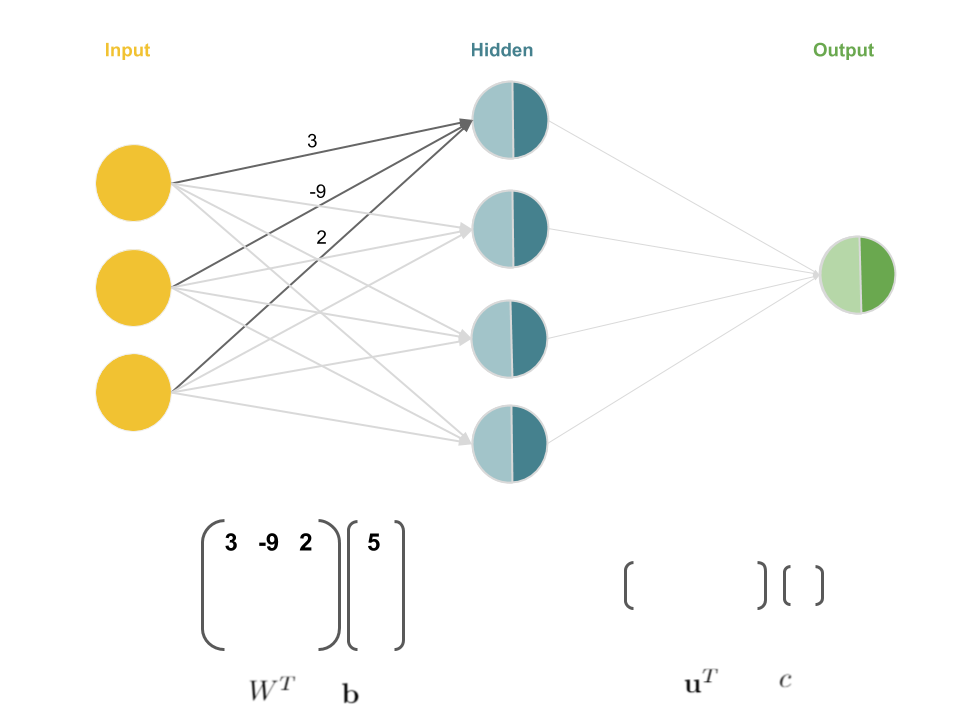
\includegraphics{plots/sinlay_one.png}}}
      \only<2>{\scalebox{1}{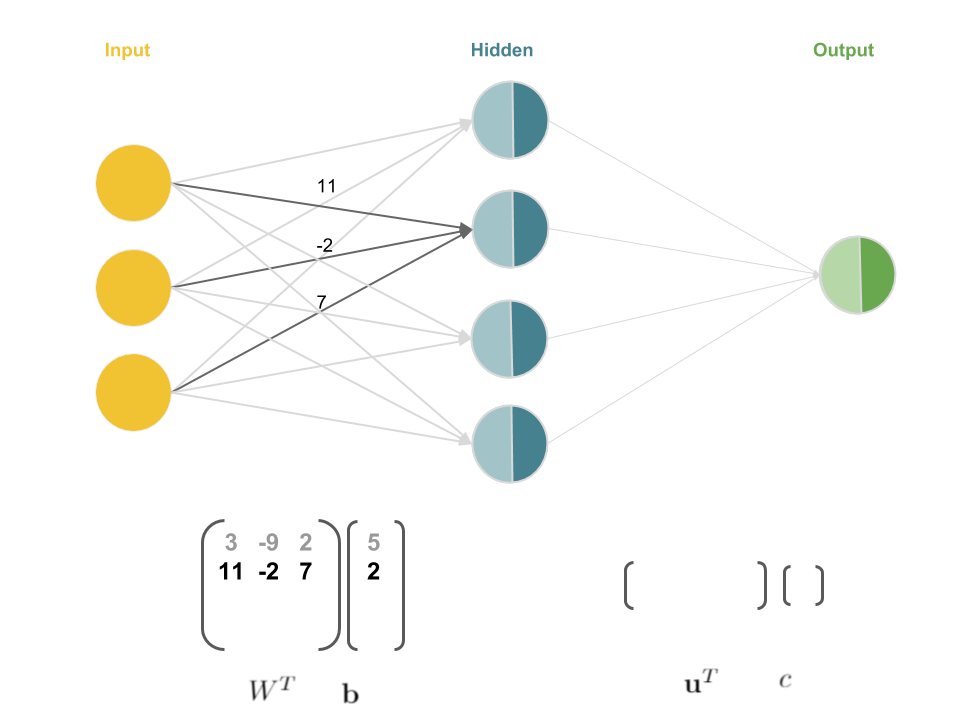
\includegraphics{plots/sinlay_two.png}}}
      \only<3>{\scalebox{1}{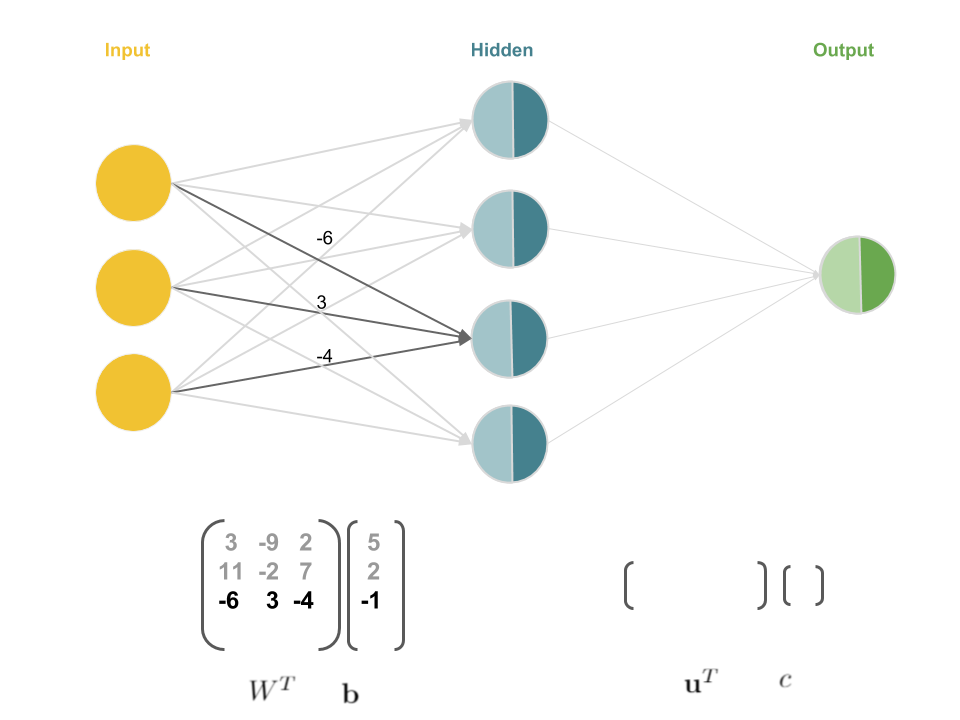
\includegraphics{plots/sinlay_three.png}}}
      \only<4>{\scalebox{1}{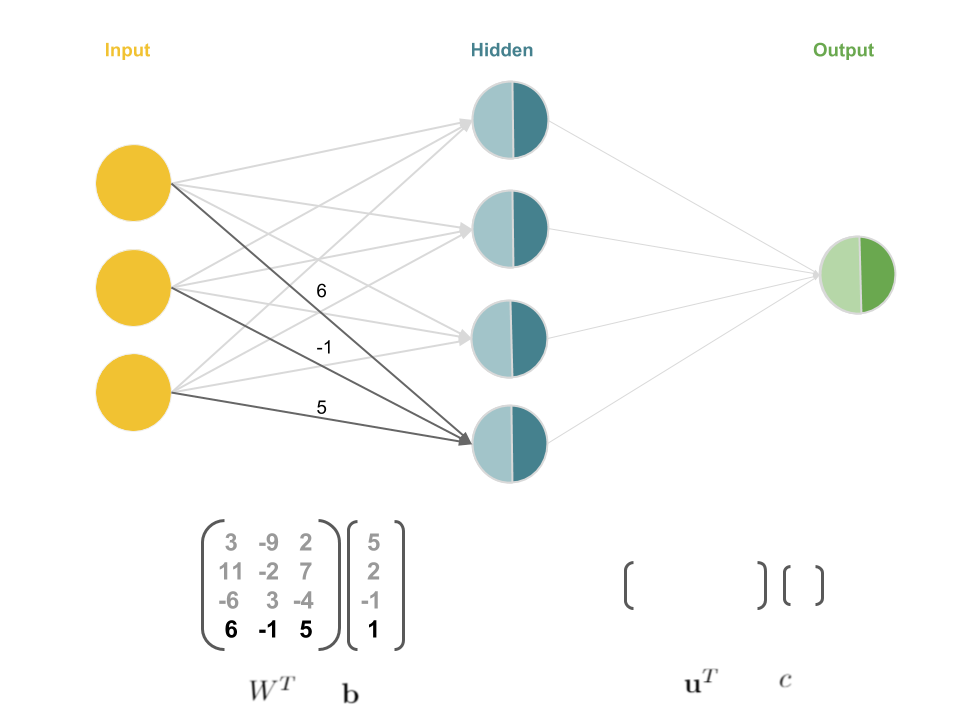
\includegraphics{plots/sinlay_four.png}}}
      \only<5>{\scalebox{1}{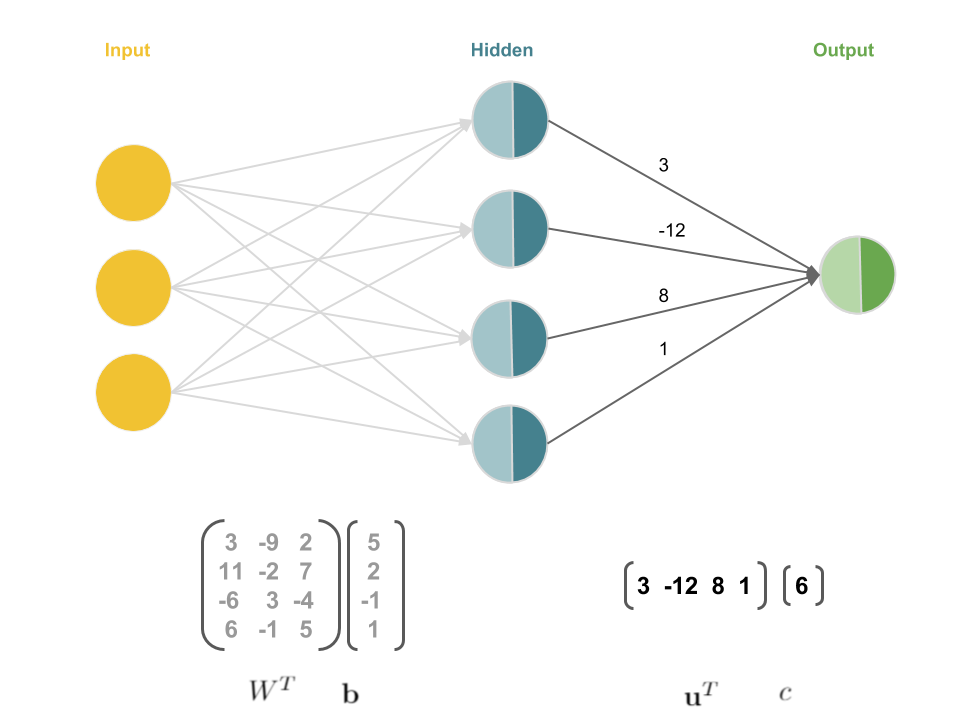
\includegraphics{plots/sinlay_five.png}}}
      \only<6>{\scalebox{1}{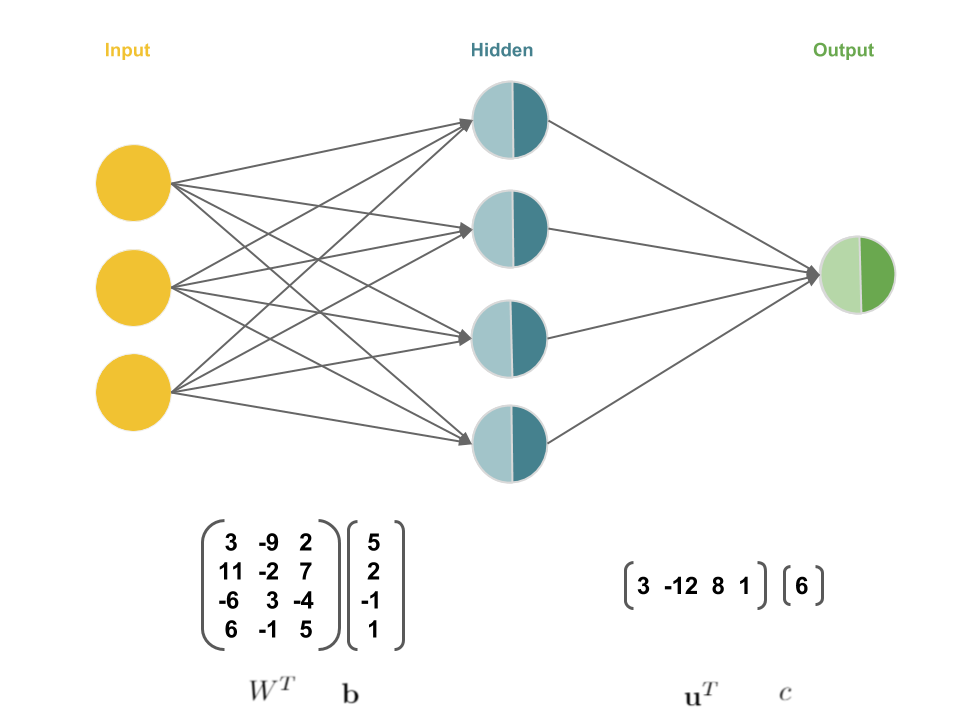
\includegraphics{plots/sinlay_six.png}}}
  \end{figure}
  \begin{figure}
    \centering
  \end{figure}
  \end{itemize}
\end{frame}
%%%%%%%%%%%%%%%%%%%%%%%%%%%%%%%%%%%%%%%%%%%%%%%%%%%%%%%%%%%%%%%%%%

\begin{frame} {Single Hidden Layer Networks: Example}
\small{Forward pass through the shallow neural network.}
  \begin{figure}
    \centering
    \only<1>{\scalebox{1}{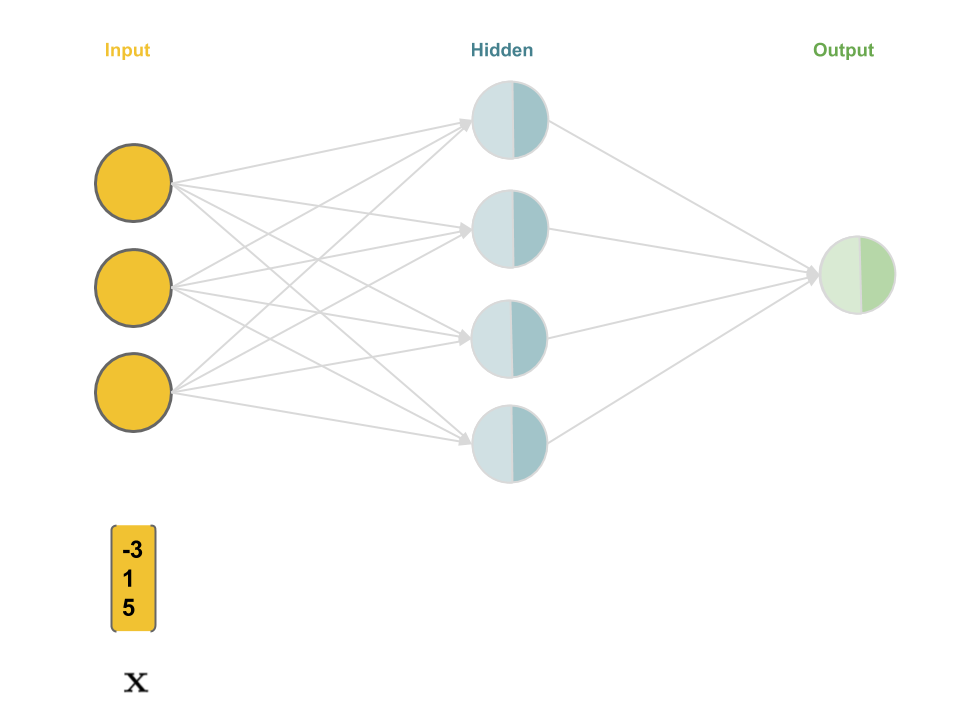
\includegraphics{plots/sinlay_seven.png}}}
    \only<2>{\scalebox{1}{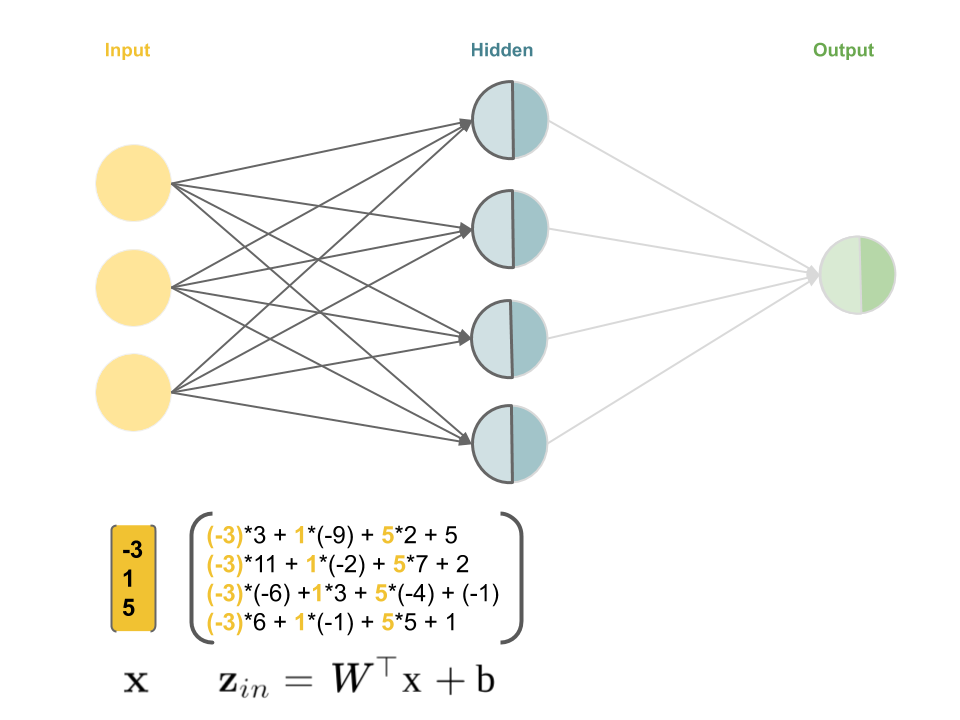
\includegraphics{plots/sinlay_eight.png}}}
    \only<3>{\scalebox{1}{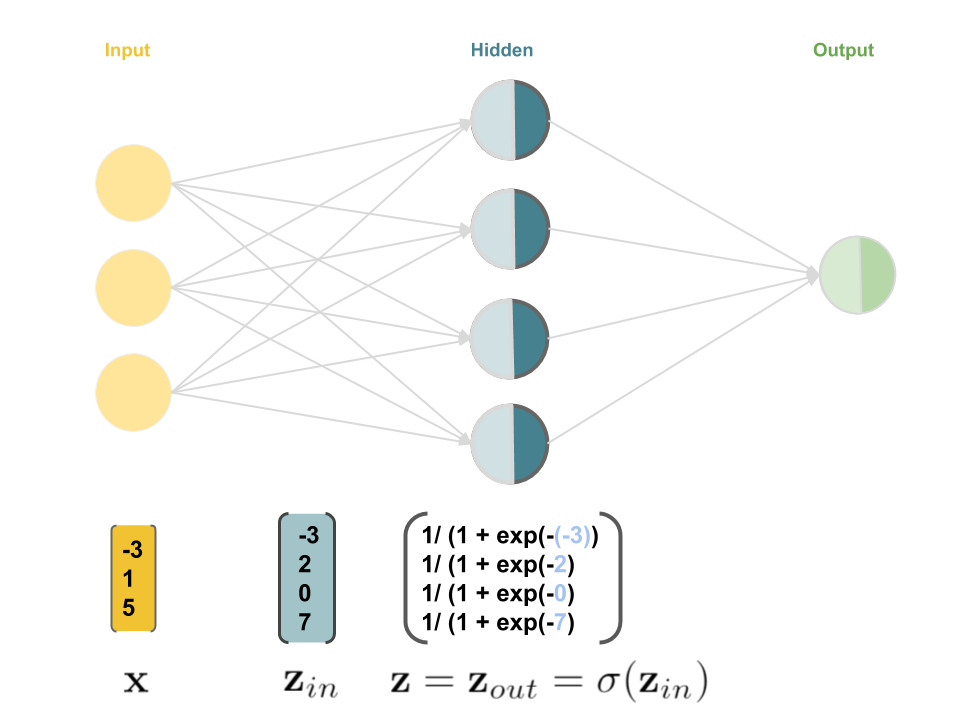
\includegraphics{plots/sinlay_nine.png}}}
    \only<4>{\scalebox{1}{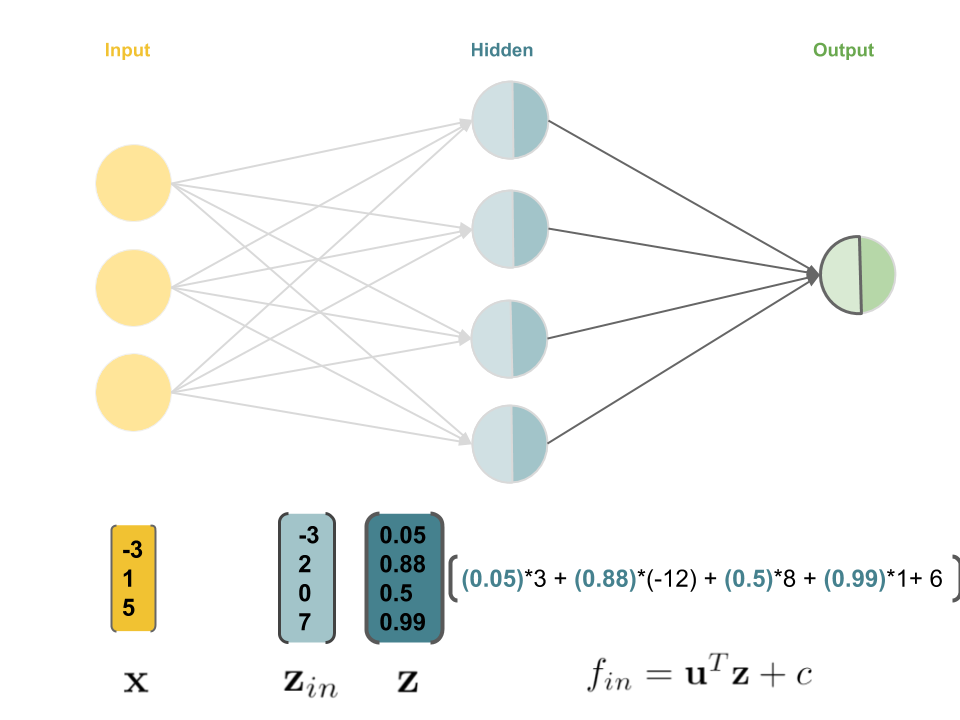
\includegraphics{plots/sinlay_ten.png}}}
    \only<5>{\scalebox{1}{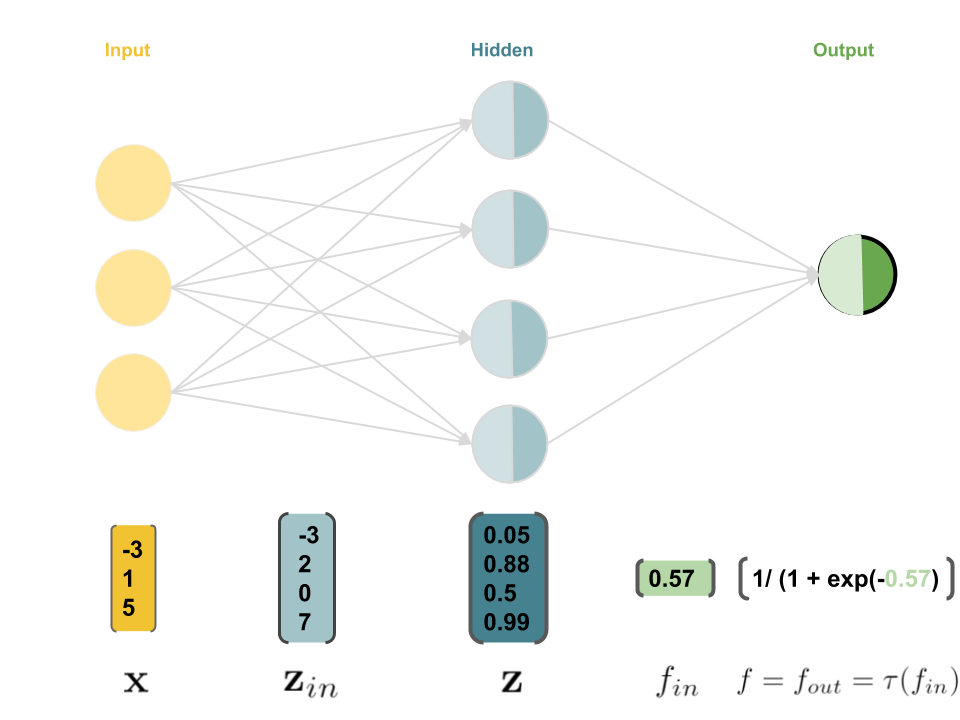
\includegraphics{plots/sinlay_eleven.png}}}
    \only<6>{\scalebox{1}{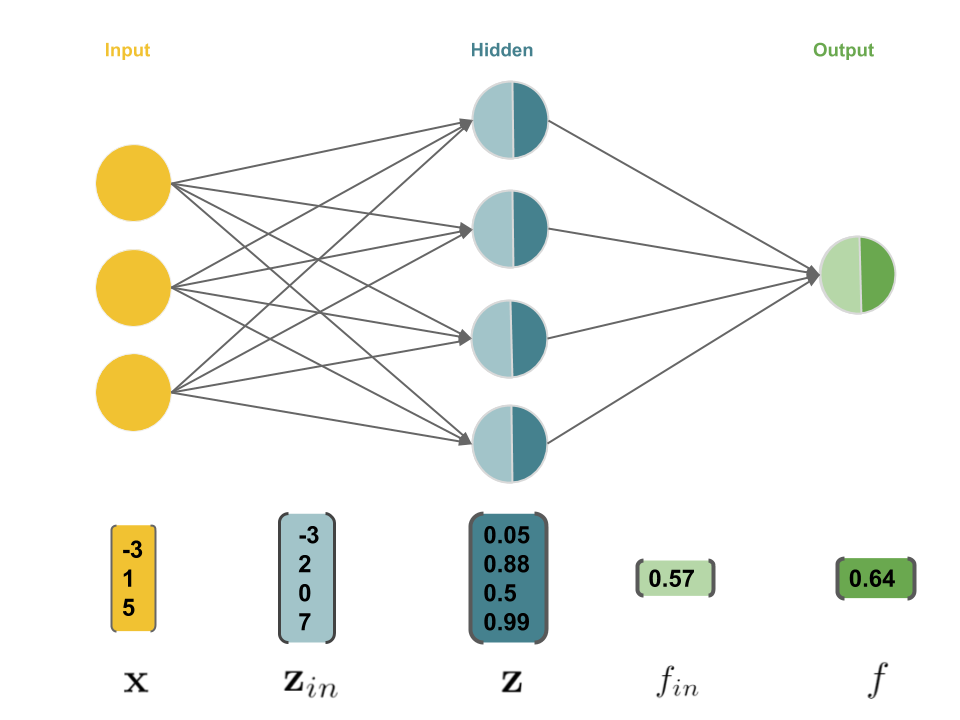
\includegraphics{plots/sinlay_twelve.png}}}
  \end{figure}
\end{frame}
%%%%%%%%%%%%%%%%%%%%%%%%%%%%%%%%%%%%%%%%%%%%%%%%%%%%%%%%%%%%%%%%%%

\begin{frame} {Hidden Layer: Activation Function}
  \begin{itemize}
    \item It is important to note that if the hidden layer does not have a non-linear activation, the network can only learn linear decision boundaries.
    \item For simplification purposes, we drop the bias terms in notation and let $\sigma = \text{id}$. Then:
    \begin{eqnarray*}
        f(\xv) & = & \tau(\wtu^\top \hidz) = \tau(\wtu^\top \sigma(\Wmat^\top \xv)) \\
         & = & \tau(\wtu^\top \sigma(\Wmat^\top \xv)) \\
         & = & \tau(\wtu^\top\Wmat^\top \xv) = \tau(\mathbf{v}^\top \xv)
      \end{eqnarray*}
      where $ \mathbf{v} = \Wmat\wtu$. It can be seen that $f(\xv)$ can only yield a linear decision boundary.
  \end{itemize}
\end{frame}
%%%%%%%%%%%%%%%%%%%%%%%%%%%%%%%%%%%%%%%%%%%%%%%%%%%%%%%%%%%%%%%%%%

\begin{frame} {Hidden Layer: Activation Function}
  \begin{blocki}{ReLU activation:}
    \item Currently the most popular choice is the ReLU (rectified linear unit):
    $$ \sigma (v) = \max(0,v) $$
  \end{blocki}
\begin{knitrout}\scriptsize
\definecolor{shadecolor}{rgb}{0.969, 0.969, 0.969}\color{fgcolor}

{\centering 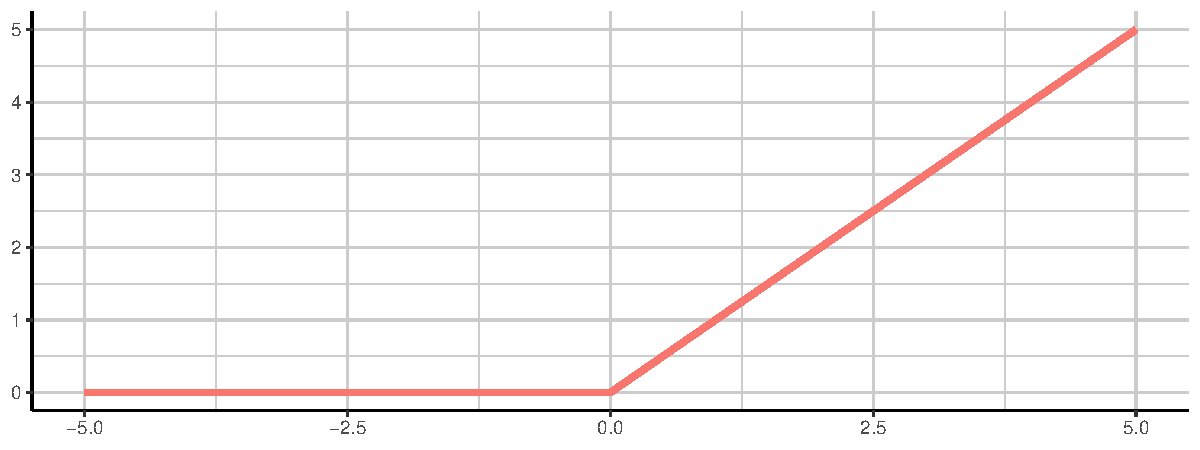
\includegraphics[width=0.95\textwidth]{figure/unnamed-chunk-2-1} 

}



\end{knitrout}
\end{frame}
%%%%%%%%%%%%%%%%%%%%%%%%%%%%%%%%%%%%%%%%%%%%%%%%%%%%%%%%%%%%%%%%%%

\begin{frame} {Hidden Layer: Activation Function}
  \begin{itemize}
    \item Some important properties of the ReLU function include:
    \item[]
    \item[]
    \begin{itemize}
      \item limits: $$\lim_{v \to -\infty} \sigma(v) = 0 \text{ and } \lim_{v \to \infty} \sigma(v) = \infty$$
      \item derivative: 
      $$\frac{\delta\sigma(v)}{\delta v} =
        \begin{cases}
                                       1 & \text{if $v > 0$} \\
                                       0 & \text{else}
        \end{cases}
      $$
    \end{itemize}
  \end{itemize}
\end{frame}
%%%%%%%%%%%%%%%%%%%%%%%%%%%%%%%%%%%%%%%%%%%%%%%%%%%%%%%%%%%%%%%%%%

\begin{frame} {Hidden Layer: Activation Function}
  \begin{blocki}{Hyperbolic tangent activation:}
    \item Another choice might be the hyperbolic tangent function:
    $$ \sigma (v) = \text{tanh}(v) = \frac{\text{sinh}(v)}{\text{cosh}(v)} = 1 - \frac{2}{\exp(2v) + 1}$$
  \end{blocki}
\begin{knitrout}\scriptsize
\definecolor{shadecolor}{rgb}{0.969, 0.969, 0.969}\color{fgcolor}

{\centering 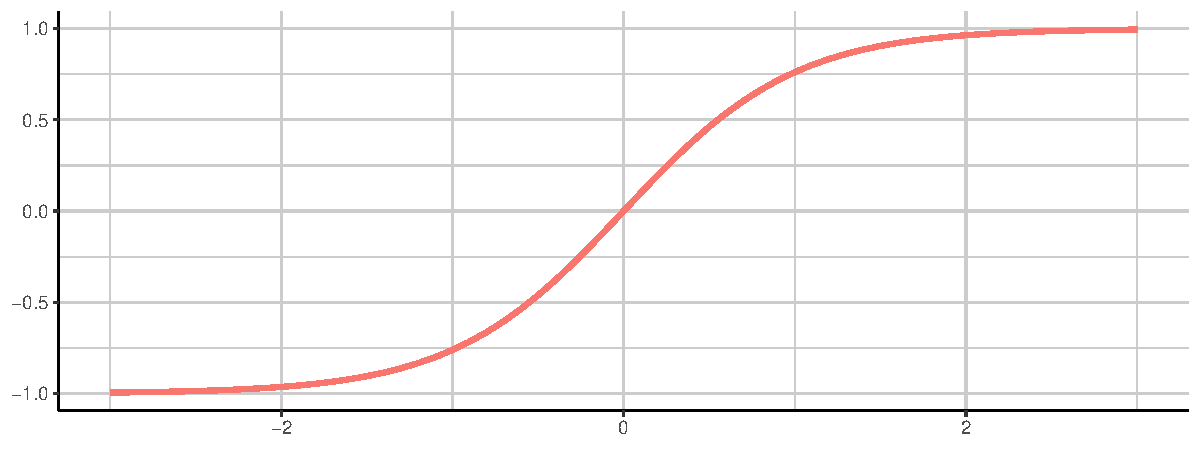
\includegraphics[width=0.95\textwidth]{figure/unnamed-chunk-3-1} 

}



\end{knitrout}
\end{frame}
%%%%%%%%%%%%%%%%%%%%%%%%%%%%%%%%%%%%%%%%%%%%%%%%%%%%%%%%%%%%%%%%%%

\begin{frame} {Hidden Layer: Activation Function}
  \begin{itemize}
    \item Some important properties of the hyperbolic tangent function include:
    \item[]
    \item[]
    \begin{itemize}
      \item limits: $$\lim_{v \to -\infty} \sigma(v) = -1 \text{ and } \lim_{v \to \infty} \sigma(v) = 1$$
      \item derivative: $$\frac{\delta\sigma(v)}{\delta v} = 1 - \text{tanh}^2(v)$$
      \item symmetry: $$\sigma(v) \text{ is rotationally symmetric about } (0, 0)$$ \\
      (that is, a rotation of $180^{\circ}$ does not change the graph of the function.)
    \end{itemize}
  \end{itemize}
\end{frame}
%%%%%%%%%%%%%%%%%%%%%%%%%%%%%%%%%%%%%%%%%%%%%%%%%%%%%%%%%%%%%%%%%%

\begin{frame} {Hidden Layer: Activation Function}
  \begin{blocki}{Sigmoid activation function:}
  \item Of course, as seen in the previous example, the sigmoid function can be used even in the hidden layer:
    $$ \sigma(v) = \frac{1}{1+\exp (-v)} $$
  \end{blocki}
\begin{knitrout}\scriptsize
\definecolor{shadecolor}{rgb}{0.969, 0.969, 0.969}\color{fgcolor}

{\centering 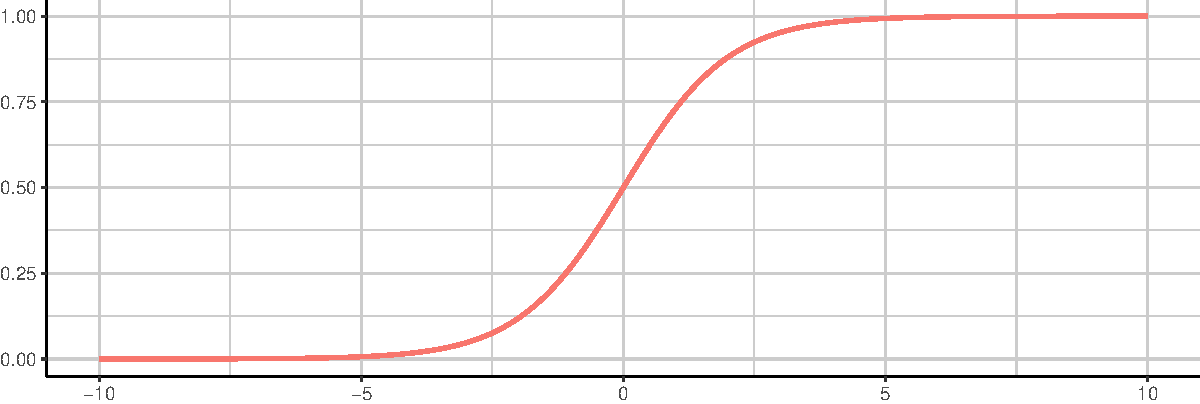
\includegraphics[width=0.95\textwidth]{figure/unnamed-chunk-4-1} 

}



\end{knitrout}
\end{frame}
%%%%%%%%%%%%%%%%%%%%%%%%%%%%%%%%%%%%%%%%%%%%%%%%%%%%%%%%%%%%%%%%%%

\begin{frame}{Hidden Layer: Activation Function}
  \begin{itemize}
    \item Some important properties of the logistic sigmoid function include:
    \item[]
    \item[]
    \begin{itemize}
      \item limits: $$\lim_{v \to -\infty} \sigma(v) = 0 \text{ and } \lim_{v \to \infty} \sigma(v) = 1$$
      \item the derivative: $$\frac{\delta\sigma(v)}{\delta v}=\frac{\exp(v)}{(1+\exp(v))^2} = \sigma(v)(1-\sigma(v))$$
      \item symmetry: $$\sigma(v) \text{ is rotationally symmetric about } (0, 0.5)$$ 
    \end{itemize}
  \end{itemize}
\end{frame}
%%%%%%%%%%%%%%%%%%%%%%%%%%%%%%%%%%%%%%%%%%%%%%%%%%%%%%%%%%%%%%%%%%


\section{Multi-Layer Feedforward Neural Networks}

\begin{vbframe}{Feedforward neural networks}
  \begin{itemize}
    \vspace{15mm}
    \item We will now extend the model class once again, such that we allow an arbitrary amount of $l$ (hidden) layers.
    \vspace{5mm}
    \item The general term for this model class is (multi-layer) \textbf{feedforward networks} (inputs are passed through the network from left to right, no feedback-loops are allowed)
\end{itemize}
\framebreak
%%%%%%%%%%%%%%%%%%%%%%%%%%%%%%%%%%%%%%%%%%%%%%%%%%%%%%%%%%%%%%%%%%
\begin{itemize}
\item We can characterize those models by the following chain structure: $$f(\xv) = \tau \circ \phi \circ \sigma^{(l)} \circ \phi^{(l)} \circ \sigma^{(l-1)} \circ \phi^{(l-1)} \circ \ldots \circ \sigma^{(1)} \circ \phi^{(1)}$$ where $\sigma^{(i)}$ and $\phi^{(i)}$ are the activation function and the weighted sum of hidden layer $i$, respectively. $\tau$ and $\phi$ are the corresponding components of the output layer.

\item Each hidden layer has: 
      \begin{itemize}
        \vspace{2mm}
        \item an associated weight matrix $\Wmat^{(i)}$, bias $\biasb^{(i)}$ and activations $\hidz^{(i)}$ for $i \in \{ 1 \ldots l\}$
        \vspace{2mm}
        \item $\hidz^{(i)} = \sigma^{(i)}(\phi^{(i)}) = \sigma^{(i)}(\Wmat^{(i)T}\hidz^{(i - 1)} + \biasb^{(i)})$ , where $\hidz^{(0)} = \xv$.
      \end{itemize}
    \vspace{5mm}
    \item Again, without non-linear activations in the hidden layers, the network can only learn linear decision boundaries.
  \end{itemize}
\framebreak
%%%%%%%%%%%%%%%%%%%%%%%%%%%%%%%%%%%%%%%%%%%%%%%%%%%%%%%%%%%%%%%%%%
  \lz
  \begin{figure}
    \centering
      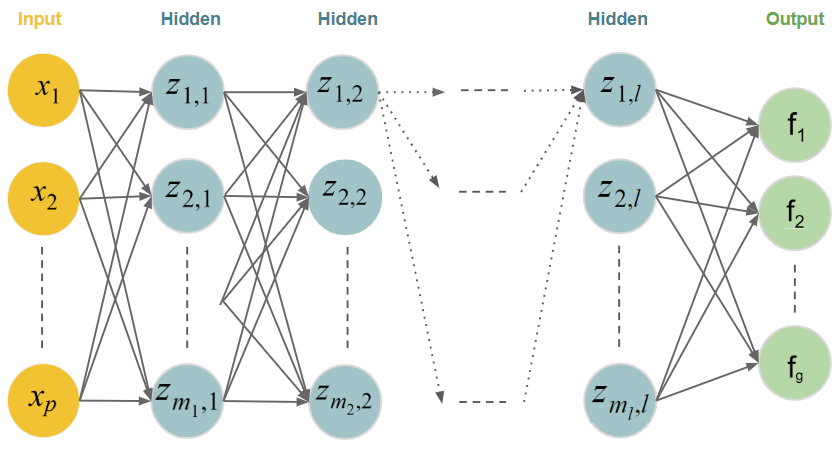
\includegraphics[width=10.5cm]{plots/deepneuralnet_new.png}
      \caption{Structure of a deep neural network with $l$ hidden layers (bias terms omitted).}
  \end{figure}
\end{vbframe}  
%%%%%%%%%%%%%%%%%%%%%%%%%%%%%%%%%%%%%%%%%%%%%%%%%%%%%%%%%%%%%%%%%%

\begin{frame} {Feedforward neural networks: Example}
  \begin{figure}
    \centering
\only<1>{\scalebox{0.95}{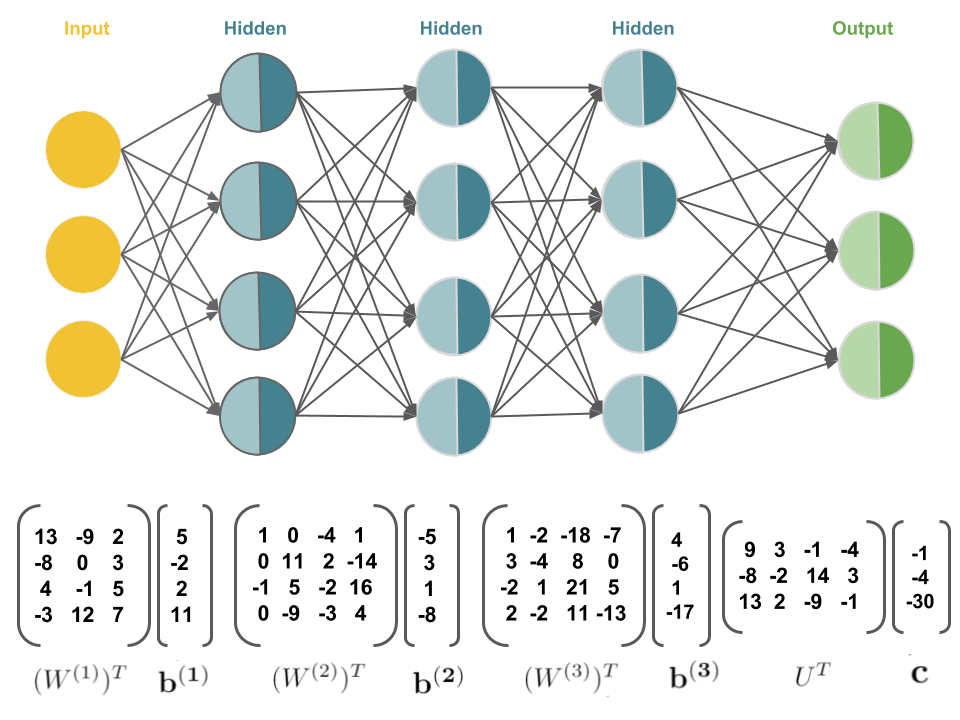
\includegraphics{plots/deepnet_one.png}}}
\only<2>{\scalebox{0.95}{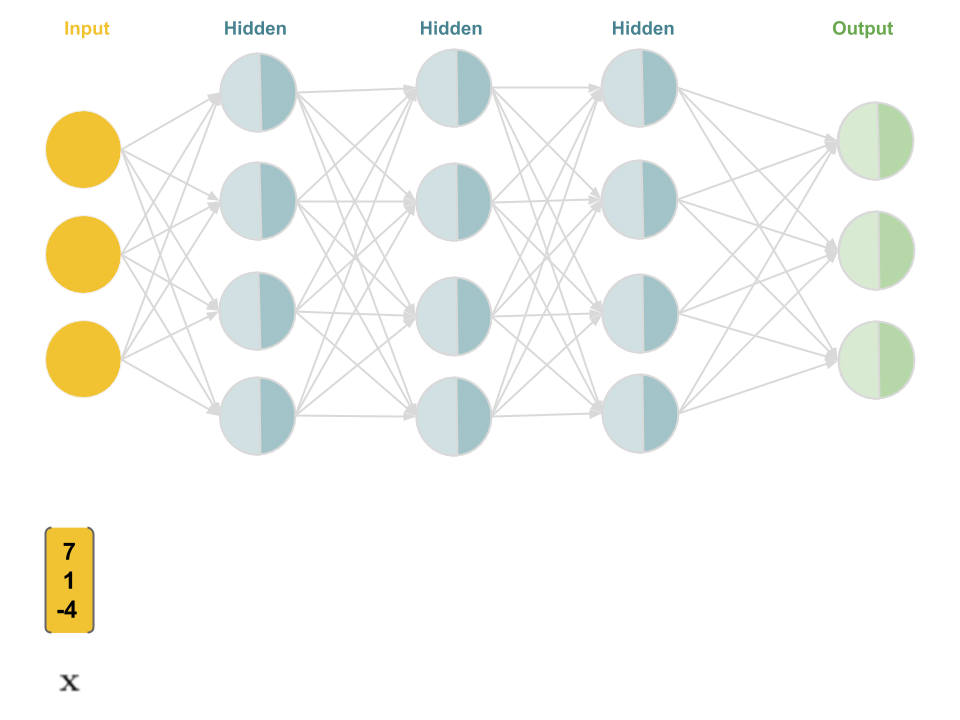
\includegraphics{plots/deepnet_two.png}}}
\only<3>{\scalebox{0.95}{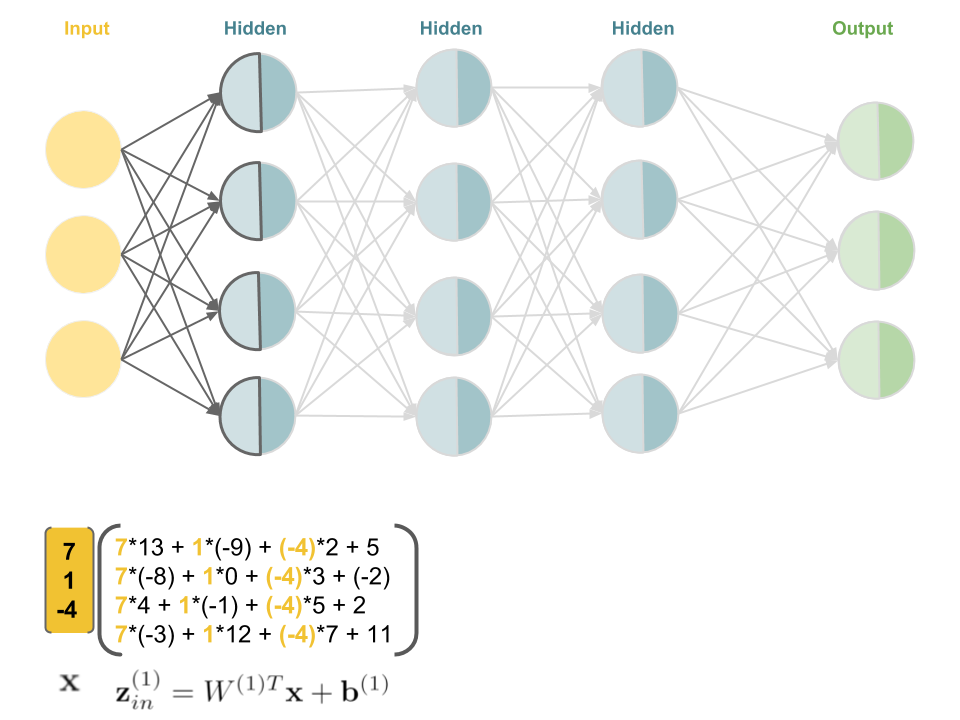
\includegraphics{plots/deepnet_three.png}}}
\only<4>{\scalebox{0.95}{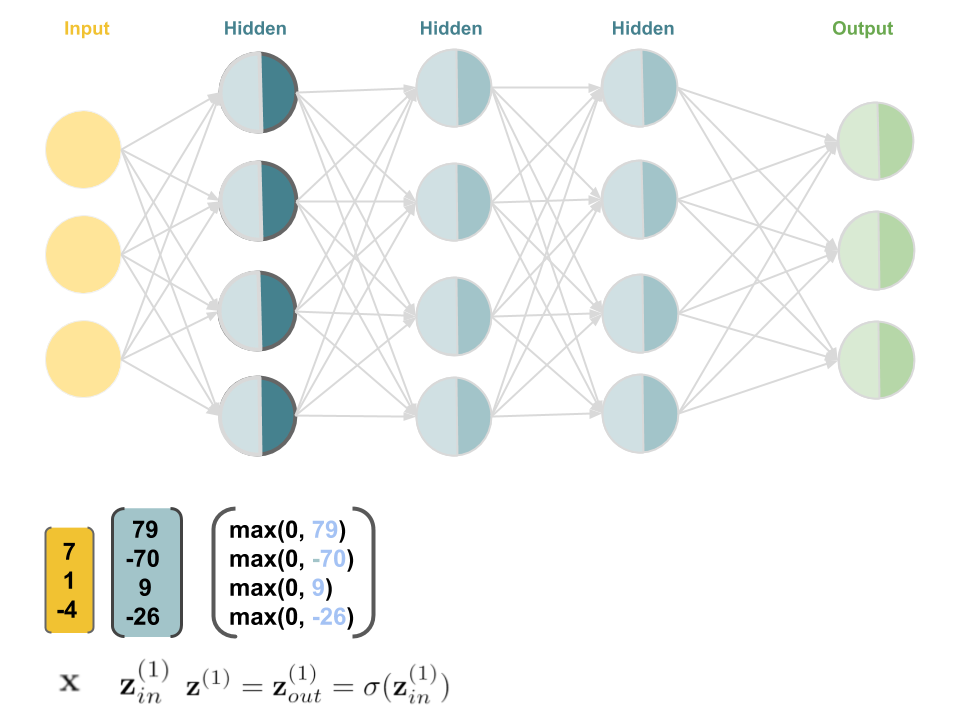
\includegraphics{plots/deepnet_four.png}}}
\only<5>{\scalebox{0.95}{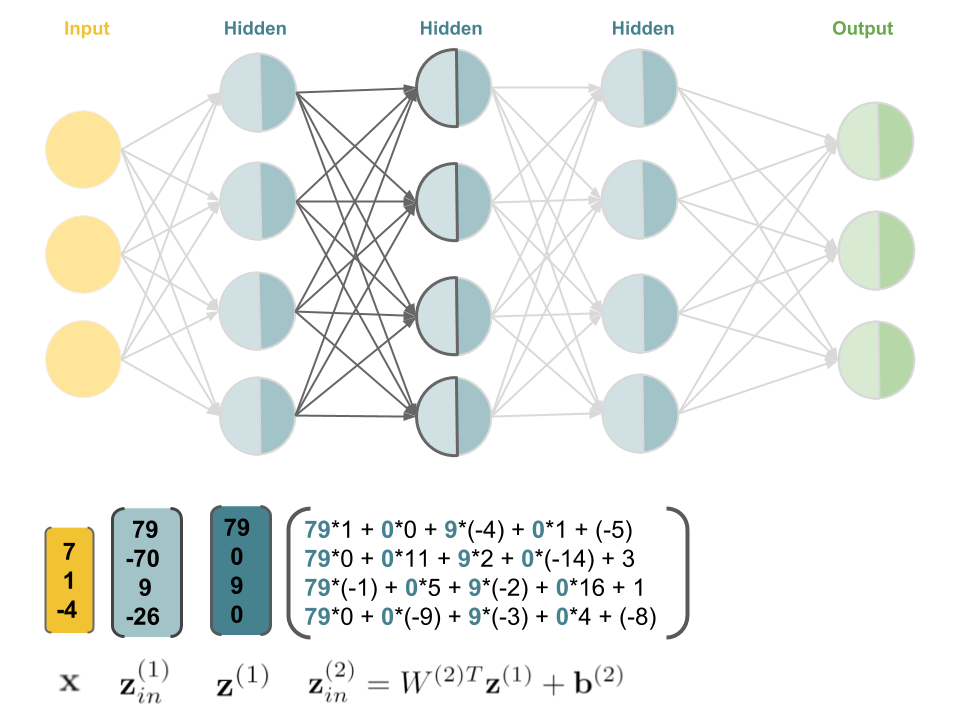
\includegraphics{plots/deepnet_five.png}}}
\only<6>{\scalebox{0.95}{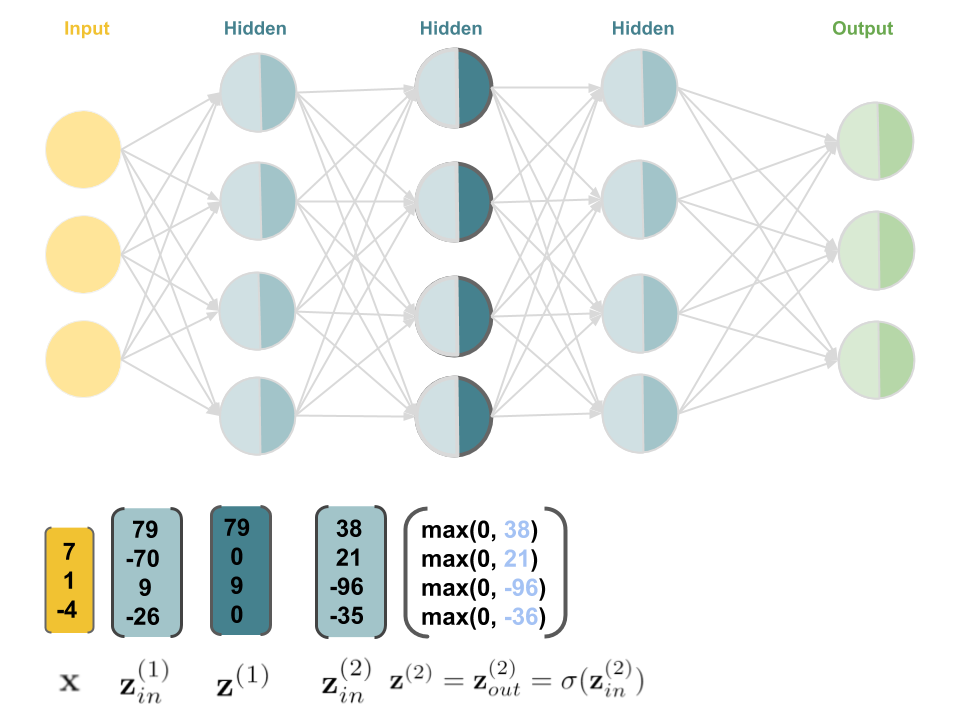
\includegraphics{plots/deepnet_six.png}}}
\only<7>{\scalebox{0.95}{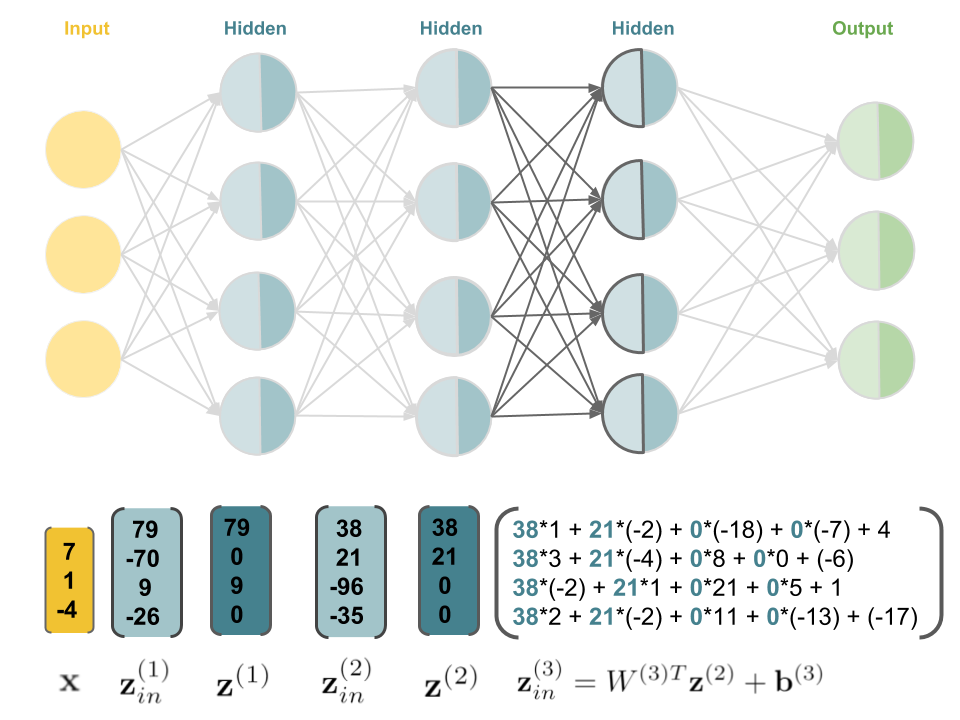
\includegraphics{plots/deepnet_seven.png}}}
\only<8>{\scalebox{0.95}{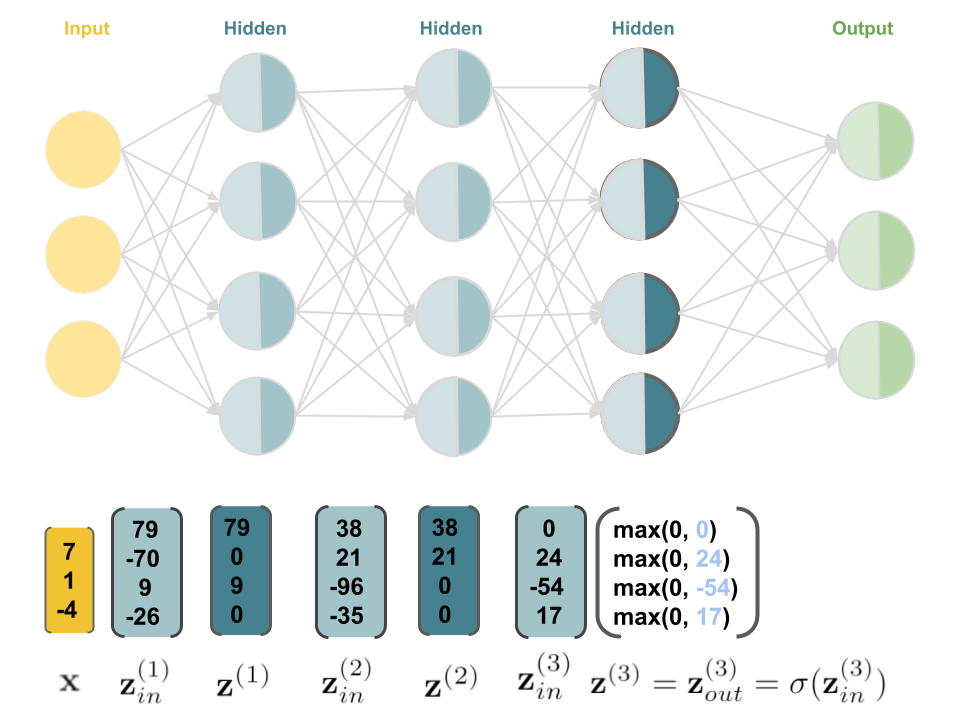
\includegraphics{plots/deepnet_eight.png}}}
\only<9>{\scalebox{0.95}{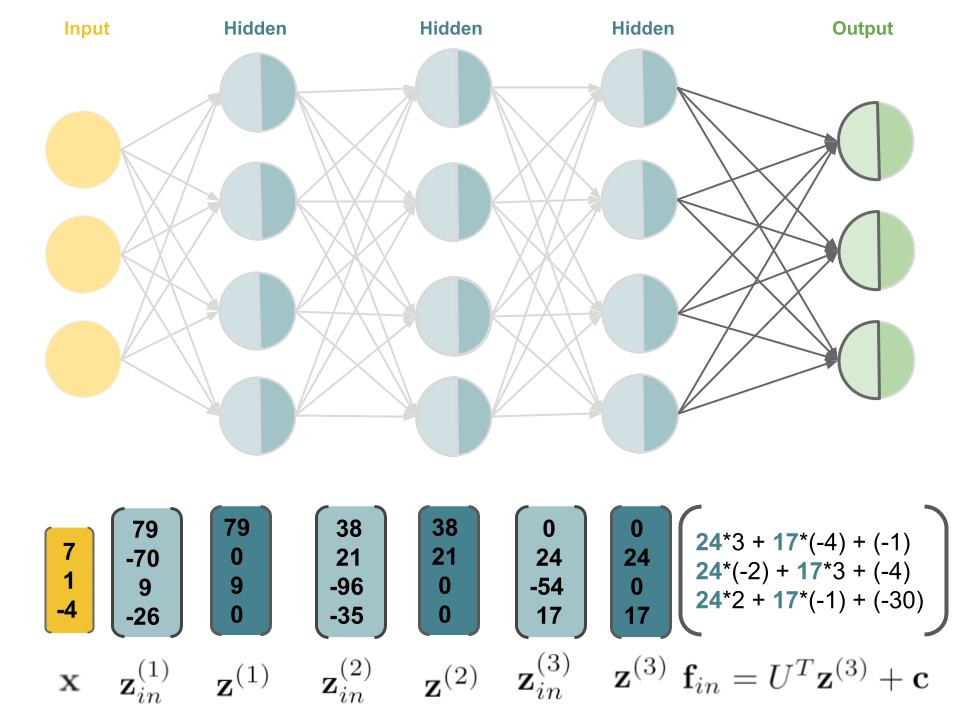
\includegraphics{plots/deepnet_nine.png}}}
\only<10>{\scalebox{0.95}{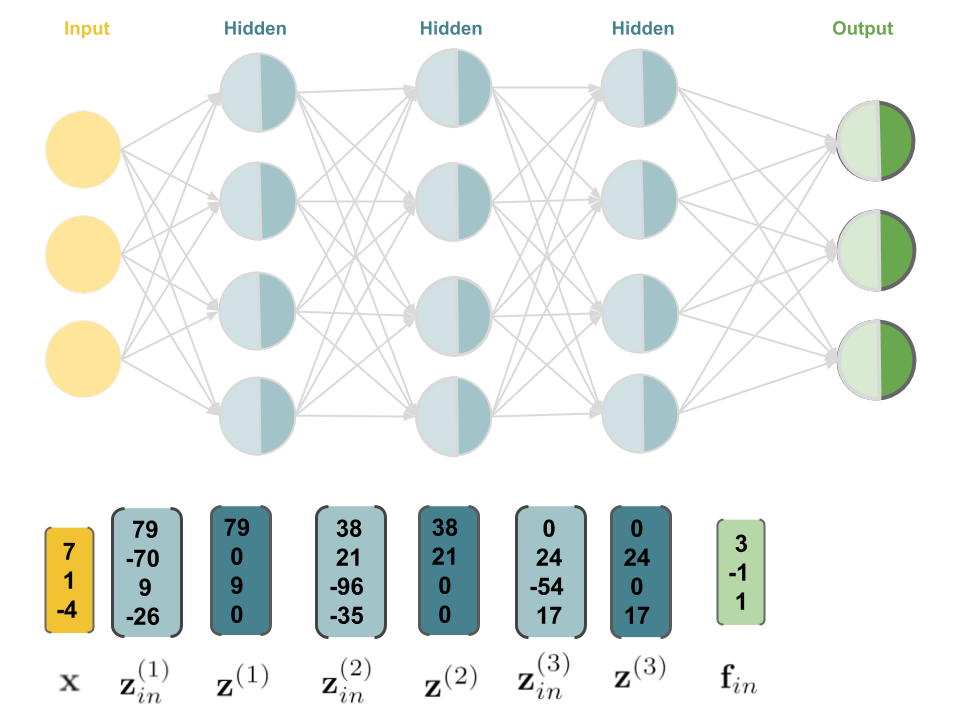
\includegraphics{plots/deepnet_ten.png}}}
\only<11>{\scalebox{0.95}{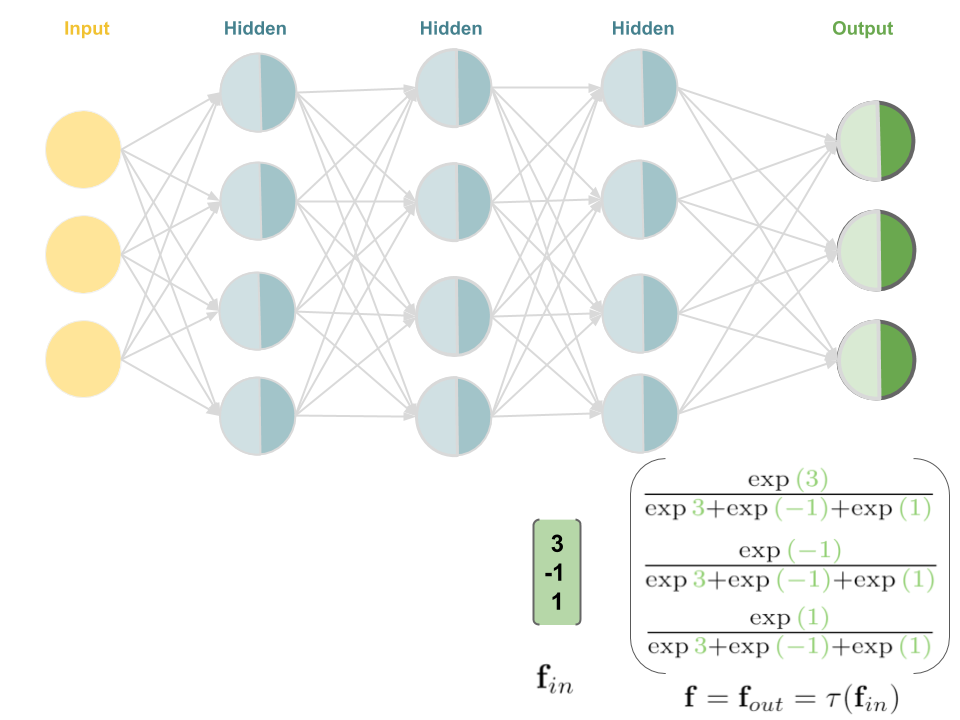
\includegraphics{plots/deepnet_eleven.png}}}
\only<12>{\scalebox{0.95}{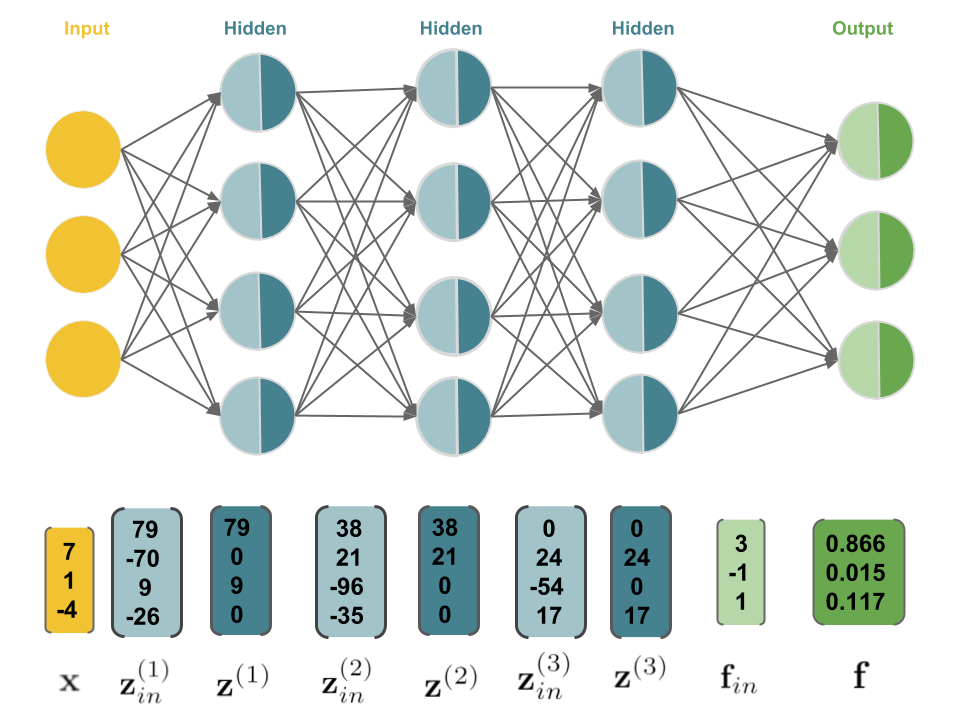
\includegraphics{plots/deepnet_twelve.png}}}
\end{figure}
\end{frame}
%%%%%%%%%%%%%%%%%%%%%%%%%%%%%%%%%%%%%%%%%%%%%%%%%%%%%%%%%%%%%%%%%%

\begin{vbframe}{Why add more layers?}
\begin{itemize}
\item Multiple layers allow for the extraction of more and more abstract representations.
\end{itemize}
\begin{figure}
\centering
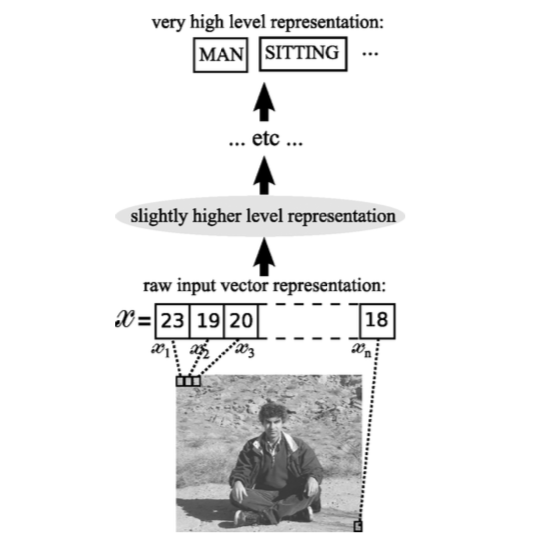
\includegraphics[width=4cm]{plots/hierachicalRepresentations.png}
\caption{Y. Bengio, Learning Deep Architectures for AI, Foundations and trends® in Machine Learning, 2009}
\end{figure}
\end{vbframe}

%%%%%%%%%%%%%%%%%%%%%%%%%%%%%%%%%%%%%%%%%%%%%%%%%%%%%%%%%%%%%%%%%%
\begin{vbframe}{Why add more layers?}
\begin{itemize}
  \item Each layer in a feed-forward neural network adds its own degree of non-linearity to the model.
\end{itemize}
  \begin{figure}
    \centering
      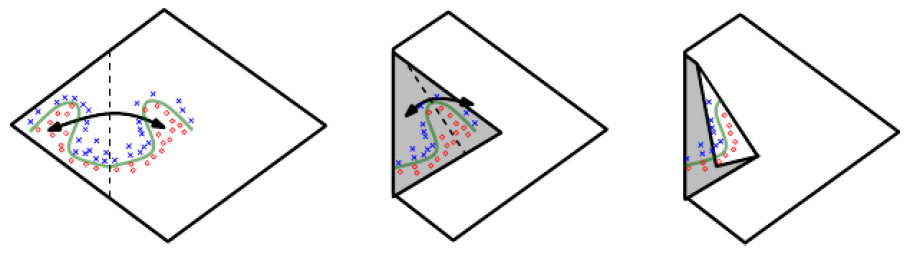
\includegraphics[width=10.5cm]{plots/folding}
      \caption{An intuitive, geometric explanation of the exponential advantage of deeper networks formally (Mont\'{u}far et al. (2014)).}
  \end{figure}
\end{vbframe}
%%%%%%%%%%%%%%%%%%%%%%%%%%%%%%%%%%%%%%%%%%%%%%%%%%%%%%%%%%%%%%%%%%

\begin{vbframe}{Deep neural networks}
  \begin{itemize}
    \item Neural networks today can have dozens or even hundreds of hidden layers. The greater the number of layers, the "deeper" the network. 
    \item Historically, deep neural networks were very challenging to train for several reasons.
    \item For one thing, the use of sigmoid activations (such as logistic sigmoid and tanh) significantly slowed down training due to a phenomenon known as \enquote{vanishing gradients}. The introduction of the ReLU activation largely solved this problem.
    \item Additionally, training deep neural networks on CPUs was too slow to be practical. Switching over to GPUs (Graphics Processing Units) cut down training time by more than an order of magnitude.
    \item Another reason neural networks were not popular until the late '00s is that when dataset sizes are small, other models (such as SVMs) and techniques (such as feature engineering) outperform them. 
    \item Therefore, the availability of large datasets (such as ImageNet) and novel architectures that are capable to handle even complex tensor-shaped data (e.g. CNNs for image data), significantly faster hardware, and equally better optimization and regularization methods made it feasible to successfully implement deep neural networks in the last decade.
    \item An increase in depth often translates to an increase in performance on a given task. 
    \item State-of-the-art neural networks, however, are much more sophisticated than the simple architectures we have encountered so far. (Stay tuned!)
    \item The term "\textbf{deep learning}" encompasses all of these developments and refers to the field as a whole.
  \end{itemize}
\end{vbframe}
%%%%%%%%%%%%%%%%%%%%%%%%%%%%%%%%%%%%%%%%%%%%%%%%%%%%%%%%%%%%%%%%%%
\endlecture
\end{document}
